%! Author = gramic
%! Date = 15.03.24

% Preamble
\clearpage
\KOMAoptions{paper=A4,paper=portrait,pagesize}
\recalctypearea
\begin{flushleft}
    \subsubsection{Patroni}
    \paragraph{Architektur}
    Ursprünglich sollte auf jedem Patroni Server (\texttt{sks1232}, \texttt{sks1233} und \texttt{sks1234}) ein \gls{etcd}-Node installiert werden.\\
    Auch sollte auf \texttt{sks1234} der \Gls{HAProxy} installiert werden.\\
    Im Kapitel \hyperref[par:patroni_installation]{Installation} wird erklärt, wieso die Architektur nun folgendermassen aussieht:
    \begin{figure}[H]
        \centering
        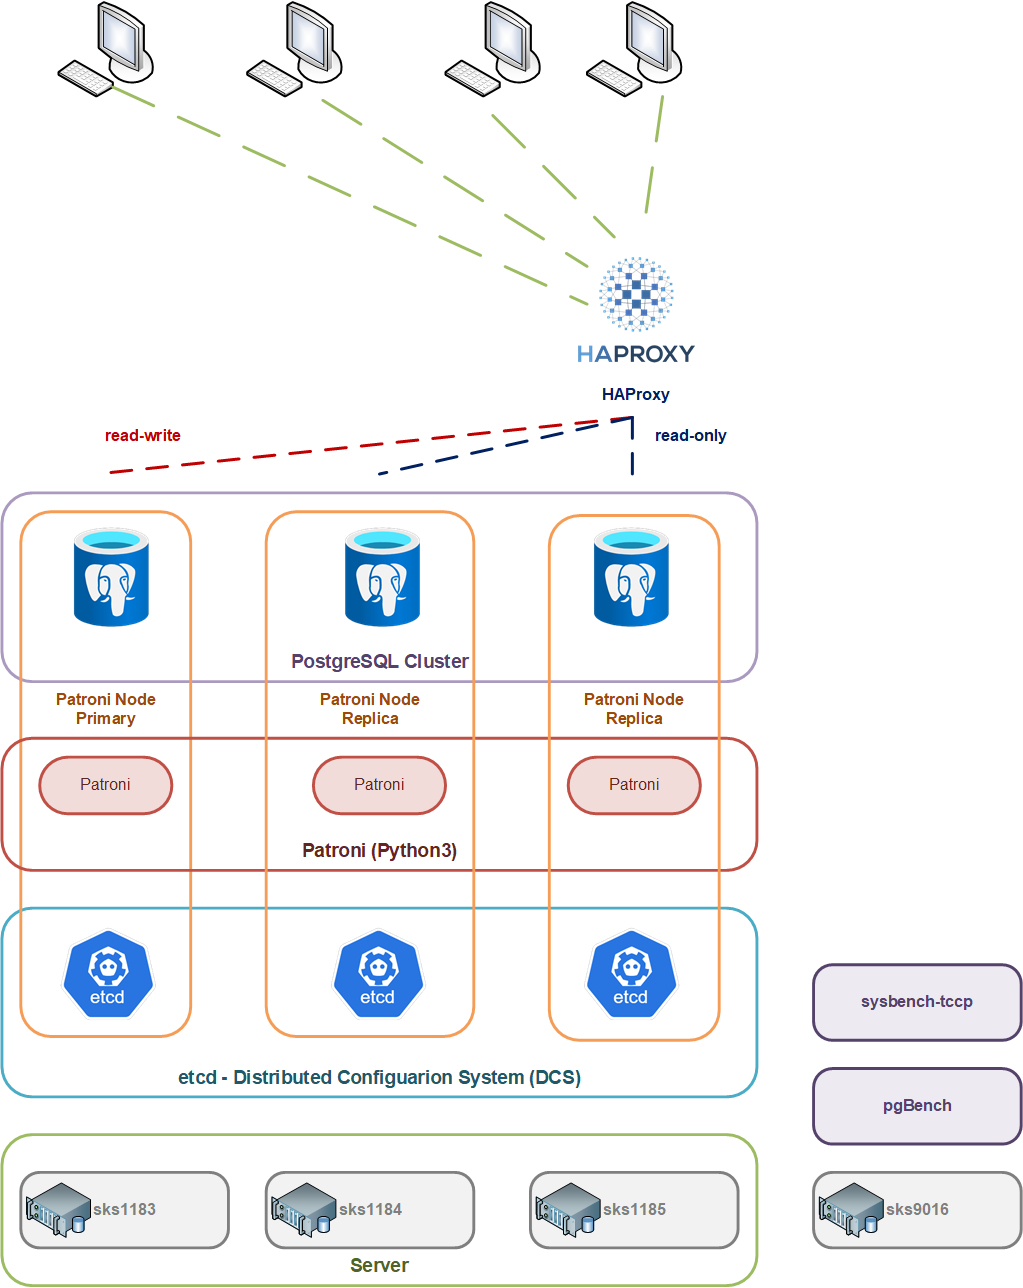
\includegraphics[width=0.8\linewidth]{source/implementation/evaluation/postgresql_ha_solutions/patroni/patroni-evaluation-architecture}
        \caption{Patroni - Evaluationsarchitektur}
        \label{fig:patroni-evaluation-architecture.png}
    \end{figure}
    Neu wird auf \texttt{sks9016} ein \gls{etcd}-Node und der \Gls{HAProxy} installiert.
\end{flushleft}
\clearpage
\KOMAoptions{paper=A4,paper=portrait,pagesize}
\recalctypearea
\begin{flushleft}
    \paragraph{Installation}
    \label{par:patroni_installation}
    Wie schon erwähnt, wurde versucht die \gls{etcd}-Nodes auf die Patroni-Nodes zu installieren.
\end{flushleft}
\clearpage
\KOMAoptions{paper=A4,paper=portrait,pagesize}
\recalctypearea
\begin{flushleft}
    Erst kam es zu einem Fehler, dass keine Verbindung zum \gls{etcd}-Node hergestellt werden konnte:
\lstset{style=gra_codestyle}
\begin{lstlisting}[language=bash, caption=Patroni - etcd API V2 Error,captionpos=b,label={lst:patroni_etcd_api_v2_error},breaklines=true]
ERROR: Failed to get list of machines from http://10.0.20.110:2379/v2: EtcdException('Bad response : 404 page not found\n')
INFO: waiting on etcd
\end{lstlisting}
    Ursache war, dass \gls{etcd} V3 ab Version v3.4 die API V2 nicht mehr per Default aktiv ist.\\
    Man könnte bis v3.7 die API V2 noch aktivieren:
\lstset{style=gra_codestyle}
\begin{lstlisting}[language=bash, caption=Patroni - etcd API V2 Enable,captionpos=b,label={lst:patroni_etcd_api_v2_enable},breaklines=true]
ETCDCTL_API=2
\end{lstlisting}
    Die nachhaltigere Lösung ist, im Konfiguations-yml-File des Patroni-Nodes Version 3 zu setzen (und dieses Package auch explizit zu installieren):
\lstset{style=gra_codestyle}
\begin{lstlisting}[language=yaml, caption=Patroni - etcd3 Flag,captionpos=b,label={lst:patroni_etcd3_flag},breaklines=true]
...
etcd3:
    host: <ip / hostname>:2379
...
\end{lstlisting}
\end{flushleft}
\clearpage
\KOMAoptions{paper=A4,paper=portrait,pagesize}
\recalctypearea
\begin{flushleft}
    Der Primary-Node konnte in jeden Fall installiert und deployt werden.\\
    Sobald aber jeweils die Replika-Nodes gestartet wurden, kam es zu einem Fehler.\\
    Die Ursache war, dass es ja bereits einen Host-Key für den jeweiligen Hostnamen resp.
    die entsprechende IP gab, nämlich den \gls{etcd}-Node.\\
    So kam es jeweils zu einem Key-Error.\\
    Nach einigem Versuchen, etwa die Keys neu zu beschreiben, brach ich die übung ab.\\
    Der \gls{etcd}-Node wurde nun nur noch auf dem Server \texttt{sks9060} installiert.\\
    Resultat war, dass der Cluster lauffähig wurde.\\
%    Daraus nehme ich für die ganze Arbeit folgende Erkenntnis heraus, wenn ein System nicht lauffähig gemacht werden kann:\\
%    \textlarger{\textit{\say{Im Zweifelsfall die Komplexität herausnehmen und das ganze System so weit vereinfachen, bis es funktioniert}}}
\end{flushleft}
\clearpage
\KOMAoptions{paper=A4,paper=portrait,pagesize}
\recalctypearea
\begin{flushleft}
    Passwörter können mit dem Bootstrap mitgegeben werden.\\
    Dazu muss im \texttt{postgresql}-Segment das Subsegment \texttt{authentication} erstellt werden.\\
    Der Replikationsuser muss mit einem subsegment \texttt{replication} und der postgres-User mit \texttt{superuser} angegeben werden:
\lstset{style=gra_codestyle}
\begin{lstlisting}[language=yaml, caption=Patroni - Passwörter,captionpos=b,label={lst:patroni_passwords},breaklines=true]
...
postgresql:
    ...
    authentication:
        replication:
            username: replicator
            password: <password>
        superuser:
            username: postgres
            password: <password>
...
\end{lstlisting}
\end{flushleft}
\clearpage
\KOMAoptions{paper=A4,paper=portrait,pagesize}
\recalctypearea
\begin{flushleft}
    Zuerst lief der Cluster nur asynchron, auch die ersten beiden Benchmarks wurden so ausgeführt.\\
    Der Cluster lässt sich nämlich nicht synchron Bootstrapen, die Konfiguration muss nachträglich gemacht werden.\\
    Dazu kann ein JSON mit den geänderten Konfiguration übergeben werden, in dieser Konfiguration musste dabei das yml-File mit der Konfiguration angegeben werden:
\lstset{style=gra_codestyle}
\begin{lstlisting}[language=bash, caption=Patroni - Synchrone Replikation setzen,captionpos=b,label={lst:patroni_set_sync_replication},breaklines=true]
patronictl -c /etc/patroni/config.yml edit-config --apply - --force <<'JSON'
{
 synchronous_mode: "on",
 synchronous_mode_strict: "on",
 synchronous_node_count: 2,
 "postgresql":
   {
   "parameters":{
     "synchronous_commit": "on",
     "synchronous_standby_names": "*"
   }
  }
}
JSON
\end{lstlisting}
\end{flushleft}
\clearpage
\KOMAoptions{paper=A4,paper=portrait,pagesize}
\recalctypearea
\begin{flushleft}
    Die Vergrösserung der Disks hat nur einen begrenzten Impact.\\
    Lediglich das Verzeichnis \texttt{pg\_wal}, welches die \texttt{WAL}-Files aufnimmt, muss angepasst werden.\\
    Um die Umstellung ohne Reinstallation durchführen zu können, muss mit symlinks gearbeitet werden.\\
    Die Daten können via Tablespace auf die grösseren mounts gesetzt werden.\\
\end{flushleft}
\clearpage
\KOMAoptions{paper=A4,paper=portrait,pagesize}
\recalctypearea
\begin{flushleft}
    Die vollständige Dokumentation der Evaluationsinstallation ist im \hyperref[subsec:evaluation_installation_patroni]{Anhang - Installation Patroni} zu finden.
\end{flushleft}